\documentclass[border=0.125cm]{standalone}
\usepackage{tikz}
\usetikzlibrary{positioning, shadows, matrix, calc}
\usepackage{numprint}
\usepackage{adjustbox}
\usepackage[first=0, last=1]{lcg}
\newcommand{\random}{\rand\arabic{rand}}
\begin{document}
\definecolor{green}{RGB}{55,111,66}
\definecolor{red}{RGB}{226,104,104}

\tikzset{%
  every neuron/.style={
    circle,
    draw,
    minimum size=1.5cm
  },
  neuron missing/.style={
    draw=none, 
    scale=2,
    text height=0.333cm,
    execute at begin node=\color{black}$\vdots$
  },
  doc/.style={
    draw, 
    minimum height=4em, 
    minimum width=3em, 
    fill=white, 
    label={[label distance=-1.15cm]30: \tiny patent},
    double copy shadow={shadow xshift=4pt, 
                    shadow yshift=4pt, 
                    fill=white, 
                    }
  },
  doc2/.style={
    draw, 
    minimum height=4em, 
    minimum width=3em, 
    fill=white, 
    label={[label distance=-1.05cm]30: \tiny html},
    double copy shadow={shadow xshift=4pt, 
                    shadow yshift=4pt, 
                    fill=white, 
                    }
  },
  doc missing/.style={
  draw=none, 
  scale=2,
  text height=0.333cm,
  execute at begin node=\color{black}$\vdots$
  },
  matr/.style={
    matrix of math nodes, 
    left delimiter={[}, 
    right delimiter={]},
    ampersand replacement=\&,
    inner sep=1pt,
  }
}


\begin{tikzpicture}[x=1.5cm, y=1.5cm, >=stealth]

% Patent documents
\foreach \m/\l [count=\y] in {doc,doc,doc,doc missing,doc}
  \node [\m] (pat-\y) at (0,3-1.25*\y) {};

% Technology classes
\foreach \m/\l [count=\y] in {1,missing,3}
  \node [every neuron/.try, neuron \m/.try ] (tech-\m) at (2,2-1.25*\y) {};
  
\foreach \m/\l [count=\y] in {Y02A, ,Y02C}
  \node (tech-\m) at (2,2-1.25*\y) {\m};

% Technology vectors
{\tiny
\foreach \m [count=\y] in {matr,doc missing,matr}
    \pgfmathsetmacro{\MyRandv}{random}
    \pgfmathsetmacro{\MyRandw}{random}
    \pgfmathsetmacro{\MyRandx}{random}
    \pgfmathsetmacro{\MyRandy}{random}
    \pgfmathsetmacro{\MyRandz}{random}
    \matrix [\m, color=green] (techvec-\y) at (4,2-1.25*\y) 
        {
        %\MyRandv \\
        \MyRandw \\
        \MyRandx \\
        \MyRandy \\
        \vdots \\
        \MyRandz \\
        };
}

% Company vectors

{\tiny
\foreach \m [count=\y] in {matr,matr,matr,matr,doc missing,matr}
    \pgfmathsetmacro{\MyRanda}{random}
    \pgfmathsetmacro{\MyRandb}{random}
    \pgfmathsetmacro{\MyRandc}{random}
    \pgfmathsetmacro{\MyRandd}{random}
    \pgfmathsetmacro{\MyRande}{random}
    \matrix [\m, color=red] (compvec-\y) at (8,3.5-1.25*\y) 
        {
        %\MyRanda \\
        \MyRandb \\
        \MyRandc \\
        \MyRandd \\
        \vdots \\
        \MyRande \\
        };
}  
% Company texts
\foreach \m/\l [count=\y] in {doc2,doc2,doc2,doc2,doc missing,doc2}
  \node [\m] (comp-\y) at (10,3.5-1.25*\y) {};


% \foreach \m [count=\y] in {1,2,3,4}
%   \node [every neuron/.try, neuron \m/.try ] (output-\m) at (4,2.5-1.25*\y) {};

% \foreach \l [count=\i] in {1,2,3,n}
%   \draw [<-] (input-\i) -- ++(-1,0)
%     node [above, midway] {$I_\l$};

% \foreach \l [count=\i] in {doc,doc,doc}
%   \draw [->] (input-\l-\i.east) -- (hidden-\i.west);

% pat2tech
\draw [->] (pat-1.east) -- (tech-1.west);
\draw [->] (pat-3.east) -- (tech-1.west);

\draw [->] (pat-2.east) -- (tech-3.west);
\draw [->] (pat-3.east) -- (tech-3.west);
\draw [->] (pat-5.east) -- (tech-3.west);

% tech2techvec
\draw [->] (tech-1.east) -- (techvec-1.west);
\draw [->] (tech-3.east) -- (techvec-3.west);

% comp2compvec
\draw [->] (comp-1.west) -- (compvec-1.east);
\draw [->] (comp-2.west) -- (compvec-2.east);
\draw [->] (comp-3.west) -- (compvec-3.east);
\draw [->] (comp-4.west) -- (compvec-4.east);
\draw [->] (comp-6.west) -- (compvec-6.east);

% techvec2compvec

% \draw [->, line width = 0.5, color=red] (compvec-1.west) -- (techvec-1.east) node [above, midway] {$0.05$};
% \draw [->, line width = 1, color=red] (compvec-2.west) -- (techvec-1.east) node [above, midway] {$0.7$};
% \draw [->, line width = 0.01, color=red] (compvec-3.west) -- (techvec-1.east) node [above, midway] {$0.01$};
% \draw [->, line width = 3, color=red] (compvec-4.west) -- (techvec-1.east) node [above, midway] {$0.9$};
% \draw [->, line width = 0.75, color=red] (compvec-6.west) -- (techvec-1.east) node [above, midway] {$0.4$}; 
% \draw [->, line width = 0.5, color=green] (compvec-1.west) -- (techvec-3.east) node [below, midway] {$0.05$};
% \draw [->, line width = 1, color=green] (compvec-2.west) -- (techvec-3.east) node [below, midway] {$0.7$};
% \draw [->, line width = 0.01, color=green] (compvec-3.west) -- (techvec-3.east) node [below, midway] {$0.01$};
% \draw [->, line width = 3, color=green] (compvec-4.west) -- (techvec-3.east) node [below, midway] {$0.9$};
% \draw [->, line width = 0.75, color=green] (compvec-6.west) -- (techvec-3.east) node [below, midway] {$0.4$}; 

% \foreach \l [count=\i] in {1,n}
%   \draw [->] (output-\i) -- ++(1,0)
%     node [above, midway] {$O_\l$};

% \foreach \i in {1,...,4}
%   \foreach \j in {1,...,2}
%     \draw [->] (input-\i) -- (hidden-\j);

% \foreach \i in {1,...,2}
%   \foreach \j in {1,...,2}
%     \draw [->] (hidden-\i) -- (output-\j);

\foreach \l [count=\x from 0] in {Patent\\documents\\ , Technology\\classes\\ \text{$t$}, Technology\\embeddings\\\text{$\bar{X_t}$} , \textbf{Technological}\\ \textbf{proximity} \\ \text{$\in [0,1]$}, Comppany\\embeddings\\\text{$\bar{Y_c}$} , Company\\texts\\ \text{$c$}}
  \node [align=center, above] at (\x*2,3) {\l};

\end{tikzpicture}
%
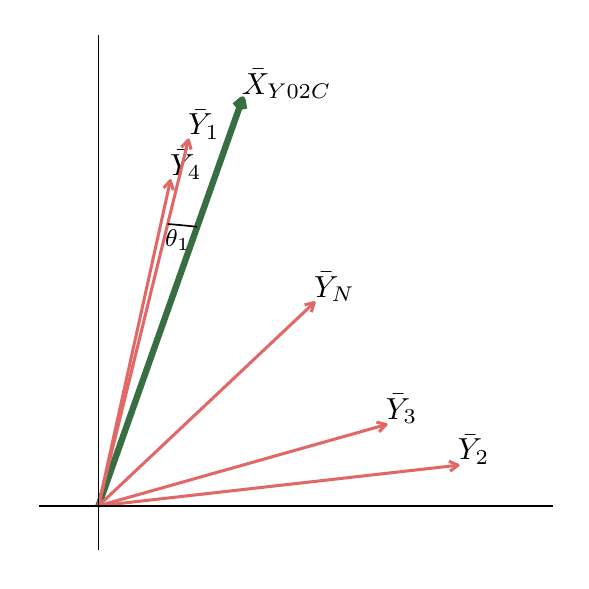
\begin{tikzpicture}[x=0.5pt,y=0.5pt]
\definecolor{fillColor}{RGB}{255,255,255}
\path[use as bounding box,fill=fillColor,fill opacity=0.00] (0,0) rectangle (385.44,385.44);
\begin{scope}
\path[clip] (  0.00,  0.00) rectangle (385.44,385.44);
\definecolor{drawColor}{RGB}{255,255,255}
\definecolor{fillColor}{RGB}{255,255,255}

\path[draw=drawColor,line width= 0.6pt,line join=round,line cap=round,fill=fillColor] (  0.00,  0.00) rectangle (385.44,385.44);
\end{scope}
\begin{scope}
\path[clip] (  8.25,  8.25) rectangle (379.94,379.94);
\definecolor{drawColor}{RGB}{0,0,0}

\node[text=drawColor,anchor=base west,inner sep=0pt, outer sep=0pt, scale=  1.10] at (154.78,337.46) {$\bar{X}_{Y02C}$};

\node[text=drawColor,anchor=base west,inner sep=0pt, outer sep=0pt, scale=  1.10] at (116.00,308.08) {$\bar{Y}_1$};

\node[text=drawColor,anchor=base west,inner sep=0pt, outer sep=0pt, scale=  1.10] at (310.95, 73.02) {$\bar{Y}_2$};

\node[text=drawColor,anchor=base west,inner sep=0pt, outer sep=0pt, scale=  1.10] at (258.96,102.40) {$\bar{Y}_3$};

\node[text=drawColor,anchor=base west,inner sep=0pt, outer sep=0pt, scale=  1.10] at (103.01,278.70) {$\bar{Y}_4$};

\node[text=drawColor,anchor=base west,inner sep=0pt, outer sep=0pt, scale=  1.10] at (206.94,190.55) {$\bar{Y}_N$};
\definecolor{drawColor}{RGB}{55,111,66}

\path[draw=drawColor,line width= 2.3pt,line join=round] ( 51.14, 39.84) -- (155.11,333.66);

\path[draw=drawColor,line width= 2.3pt,line join=round] (156.43,326.56) --
	(155.11,333.66) --
	(149.61,328.97);
\definecolor{drawColor}{RGB}{226,104,104}

\path[draw=drawColor,line width= 1.1pt,line join=round] ( 51.14, 39.84) -- (116.12,304.28);

\path[draw=drawColor,line width= 1.1pt,line join=round] (118.13,297.34) --
	(116.12,304.28) --
	(111.12,299.06);

\path[draw=drawColor,line width= 1.1pt,line join=round] ( 51.14, 39.84) -- (311.06, 69.22);

\path[draw=drawColor,line width= 1.1pt,line join=round] (305.25, 64.93) --
	(311.06, 69.22) --
	(304.44, 72.11);

\path[draw=drawColor,line width= 1.1pt,line join=round] ( 51.14, 39.84) -- (259.08, 98.60);

\path[draw=drawColor,line width= 1.1pt,line join=round] (254.04, 93.42) --
	(259.08, 98.60) --
	(252.07,100.38);

\path[draw=drawColor,line width= 1.1pt,line join=round] ( 51.14, 39.84) -- (103.12,274.90);

\path[draw=drawColor,line width= 1.1pt,line join=round] (105.30,268.01) --
	(103.12,274.90) --
	( 98.24,269.57);

\path[draw=drawColor,line width= 1.1pt,line join=round] ( 51.14, 39.84) -- (207.09,186.75);

\path[draw=drawColor,line width= 1.1pt,line join=round] (205.01,179.83) --
	(207.09,186.75) --
	(200.06,185.09);
\definecolor{drawColor}{RGB}{0,0,0}

\path[draw=drawColor,line width= 0.6pt,line join=round] (122.50,241.52) --
	(115.43,242.28) --
	(108.32,242.96) --
	(101.20,243.56);

\path[draw=drawColor,line width= 0.6pt,line join=round] (  8.25, 39.84) -- (379.94, 39.84);

\path[draw=drawColor,line width= 0.6pt,line join=round] ( 51.14,  8.25) -- ( 51.14,379.94);

\node[text=drawColor,anchor=base,inner sep=0pt, outer sep=0pt, scale=  1.10] at (108.32,227.02) {\footnotesize $\theta_1$};
\end{scope}
\end{tikzpicture}
%
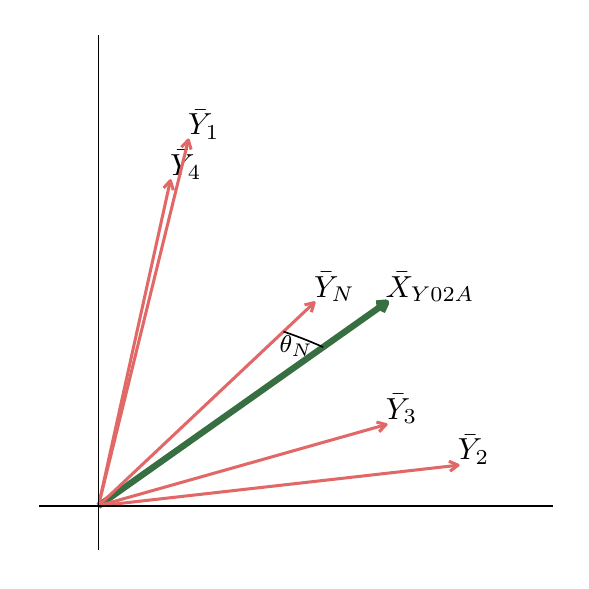
\begin{tikzpicture}[x=0.5pt,y=0.5pt]
\definecolor{fillColor}{RGB}{255,255,255}
\path[use as bounding box,fill=fillColor,fill opacity=0.00] (0,0) rectangle (385.44,385.44);
\begin{scope}
\path[clip] (  0.00,  0.00) rectangle (385.44,385.44);
\definecolor{drawColor}{RGB}{255,255,255}
\definecolor{fillColor}{RGB}{255,255,255}

\path[draw=drawColor,line width= 0.6pt,line join=round,line cap=round,fill=fillColor] (  0.00,  0.00) rectangle (385.44,385.44);
\end{scope}
\begin{scope}
\path[clip] (  8.25,  8.25) rectangle (379.94,379.94);
\definecolor{drawColor}{RGB}{0,0,0}

\node[text=drawColor,anchor=base west,inner sep=0pt, outer sep=0pt, scale=  1.10] at (258.75,190.55) {$\bar{X}_{Y02A}$};

\node[text=drawColor,anchor=base west,inner sep=0pt, outer sep=0pt, scale=  1.10] at (116.00,308.08) {$\bar{Y}_1$};

\node[text=drawColor,anchor=base west,inner sep=0pt, outer sep=0pt, scale=  1.10] at (310.95, 73.02) {$\bar{Y}_2$};

\node[text=drawColor,anchor=base west,inner sep=0pt, outer sep=0pt, scale=  1.10] at (258.96,102.40) {$\bar{Y}_3$};

\node[text=drawColor,anchor=base west,inner sep=0pt, outer sep=0pt, scale=  1.10] at (103.01,278.70) {$\bar{Y}_4$};

\node[text=drawColor,anchor=base west,inner sep=0pt, outer sep=0pt, scale=  1.10] at (206.94,190.55) {$\bar{Y}_N$};
\definecolor{drawColor}{RGB}{55,111,66}

\path[draw=drawColor,line width= 2.3pt,line join=round] ( 51.14, 39.84) -- (259.08,186.75);

\path[draw=drawColor,line width= 2.3pt,line join=round] (256.05,180.19) --
	(259.08,186.75) --
	(251.88,186.09);
\definecolor{drawColor}{RGB}{226,104,104}

\path[draw=drawColor,line width= 1.1pt,line join=round] ( 51.14, 39.84) -- (116.12,304.28);

\path[draw=drawColor,line width= 1.1pt,line join=round] (118.13,297.34) --
	(116.12,304.28) --
	(111.12,299.06);

\path[draw=drawColor,line width= 1.1pt,line join=round] ( 51.14, 39.84) -- (311.06, 69.22);

\path[draw=drawColor,line width= 1.1pt,line join=round] (305.25, 64.93) --
	(311.06, 69.22) --
	(304.44, 72.11);

\path[draw=drawColor,line width= 1.1pt,line join=round] ( 51.14, 39.84) -- (259.08, 98.60);

\path[draw=drawColor,line width= 1.1pt,line join=round] (254.04, 93.42) --
	(259.08, 98.60) --
	(252.07,100.38);

\path[draw=drawColor,line width= 1.1pt,line join=round] ( 51.14, 39.84) -- (103.12,274.90);

\path[draw=drawColor,line width= 1.1pt,line join=round] (105.30,268.01) --
	(103.12,274.90) --
	( 98.24,269.57);

\path[draw=drawColor,line width= 1.1pt,line join=round] ( 51.14, 39.84) -- (207.09,186.75);

\path[draw=drawColor,line width= 1.1pt,line join=round] (205.01,179.83) --
	(207.09,186.75) --
	(200.06,185.09);
\definecolor{drawColor}{RGB}{0,0,0}

\path[draw=drawColor,line width= 0.6pt,line join=round] (213.51,154.56) --
	(209.59,156.30) --
	(205.60,157.99) --
	(201.56,159.65) --
	(197.47,161.26) --
	(193.32,162.82) --
	(189.12,164.34) --
	(184.87,165.81);

\path[draw=drawColor,line width= 0.6pt,line join=round] (  8.25, 39.84) -- (379.94, 39.84);

\path[draw=drawColor,line width= 0.6pt,line join=round] ( 51.14,  8.25) -- ( 51.14,379.94);

\node[text=drawColor,anchor=base,inner sep=0pt, outer sep=0pt, scale=  1.10] at (194.10,150.63) {\footnotesize $\theta_N$};
\end{scope}
\end{tikzpicture}





\end{document}